\documentclass[xcolor=dvipsnames,notes]{beamer}
\usecolortheme[named=Brown]{structure}
\usetheme{default}
\setbeamertemplate{navigation symbols}{} 
\usepackage{tikz}
\usetikzlibrary{arrows,decorations.pathmorphing,backgrounds,positioning,fit}
\usetikzlibrary{datavisualization.formats.functions}
\usetikzlibrary{shapes}
\usetikzlibrary{calc,patterns,angles,quotes}
\include{macro}
\usepackage{epsfig}
\usepackage{natbib}
\usepackage{graphicx}
\usepackage{multimedia}
\usepackage{verbatim}
\include{acmmacro}
\begin{document}
%\setbeamercolor{titlelike}{fg=gray,bg=white}
%\setbeamercolor{itemize item}{fg=gray,bg=white}
%\setbeamercolor{enumerate item}{fg=gray,bg=white}
%\setbeamercolor{block title}{fg=black,bg=white}
%==============================================
\title{TPG4190 Seismic data acquisition and processing \\
               Lecture 19: First Arrival Tomography (FAT)}
\author{B. Arntsen}
\institute[NTNU]{
  NTNU\\
  Department of Geoscience and petroleum \\
  \texttt{borge.arntsen@ntnu.no}
}
\date{Trondheim fall 2020}
\begin{frame}
 \titlepage
\end{frame}
%
%======================================================
\begin{frame}{Travel-Time tomography}
%======================================================
\begin{itemize}
   \item Velocity can be estimated from measured traveltimes
   \item Here we only consider First Arrival Tomography
\end{itemize}
\end{frame}
%======================================================
\begin{frame}{Travel-time Tomography}
%======================================================

The traveltime $T$ of a seismic event can be related to
the velocity by the general equation
\begin{eqnarray}
t = \int d\sigma \frac{1}{c(\xx)}.
\end{eqnarray}
Here $c(\xx)$ is the velocity and the integration is
carried out along a ray from the source position to
the receiver position.

For constant velocity $c(\xx)=c_0$ this is simply
\begin{eqnarray}
t = \sigma/c_0,
\end{eqnarray}
where $\sigma$ is the length of the raypath.

If $c(\xx)$ is unknown we can try to solve for $c(\xx)$
\begin{eqnarray}
t_i(\xx_r) = \int d\sigma_i \frac{1}{c(\xx)},
\end{eqnarray}
where the subscript $i$ indicates different raypaths through the same model.
This equation is possible to solve, but will be non-linear because the raypath
will change with velocity and is in general unknown.
\end{frame}
%
%======================================================
\begin{frame}{Travel-time Tomography}
%======================================================
We will limit ourselves to the case where we do not have reflected
waves but only Diving waves or refracted waves. 
The general approach to find the velcity $c(\xx)$ can be formulated as
an optimization problem:

Find the velocity $c(x)$ which minimizes 
\begin{eqnarray}
E(\ww)=\frac{1}{2}\sum_{i=1,N_r}(t_i - t^{obs}_i)^2
\end{eqnarray}
where 
\begin{itemize}
  \item $t^{obs}_i$: Observed (measured) traveltime for receiver no $i$.
  \item $t_i$:   Modeled (simulated) traveltime for receiver no $i$.
  \item $N_r$: No of receivers.
  \item $w=1/c^2$: is the squared slowness 
\end{itemize}
\end{frame}
%
%======================================================
\begin{frame}{Travel-time Tomography}
%======================================================
First Arrival Rays
\begin{figure}
  \includegraphics[width=\textwidth]{Fig/fig1.png}
\end{figure}
\end{frame}
%======================================================
\begin{frame}{Travel-time Tomography}
%======================================================
It is customary to denote the traveltimes (observed and simulated)
using a vector
\begin{eqnarray}
  \ttt_i & = & (t_1,t_2,\ldots,t_{N_r}),\\
  \ttt^{obs}_i & = & (t^{obs}_1, t^{obs}_2,\ldots,t^{obs}_{N_r}),
\end{eqnarray}
Also the slowness is considered a vector
\begin{eqnarray}
  \ww = (w_1,w_2,\ldots,w_{N}),
\end{eqnarray}
where each index $i$ refers to a position in the model. $N$ is the
total number of unknown slowness values.
and the Error $E$ is written
\begin{eqnarray}
  E(\ww) = (\ttt-\ttt^{obs})^T(\ttt-\ttt^{obs}) 
\end{eqnarray}
\end{frame}
%======================================================
\begin{frame}{Travel-time Tomography}
%======================================================
We use a Taylor expansion around a known point $\ww$
\begin{eqnarray}
  E(\ww+\delta\ww) = E(\ww)+\delta\ww^T\nabla_w E(\ww) +
                     \frac{1}{2}\delta\ww^T\HH(\ww)\delta\ww + \ldots,
\end{eqnarray}
where $\delta\ww$ is a small deviation from $\ww$.
The gradient $\nabla_w$ is defined by
\begin{eqnarray}
  \nabla_w E(\ww) = \frac{\partial E}{\partial \ww} = \JJ^T(\ttt-\ttt^{obs})
\end{eqnarray}
and
\begin{eqnarray}
J_{ij} = \frac{\partial E}{\partial w_j} = 
           (t_i-t^{obs}_i)\frac{\partial t_i}{\partial w_j}
\end{eqnarray}
\end{frame}
%======================================================
\begin{frame}{Travel-time Tomography}
%======================================================
The Hess matrix $\HH$ can be approximated with
%
\begin{eqnarray}
\HH = \JJ^T\JJ.
\end{eqnarray}
%
At the solution point we have $E(\ww+\delta\ww)=0$ and the condition
$\nabla_{\delta\ww}E(\ww+\delta\ww) = 0$ leads to the least-squares equation
\begin{eqnarray}
  \JJ^T(\ttt-\ttt^{obs}) = \left(\JJ^T\JJ\right)\delta\ww
\end{eqnarray}
This equation can be solved for the squared slowness $\ww$.
The traveltime vector $\ttt$ is found by solving the Eikonal equation.
The Gradient of $E$ can also be found by making use of the Eikonal equation.
\end{frame}
%======================================================
\begin{frame}{Travel-time Tomography}
%======================================================
First Arrival Rays
\begin{figure}
  \includegraphics[width=\textwidth]{Fig/figa.png}
\end{figure}
\end{frame}
%======================================================
\begin{frame}{Travel-time Tomography}
%======================================================
First Arrival Rays
\begin{figure}
  \includegraphics[width=0.8\textwidth]{Fig/figb.png}
\end{figure}
\end{frame}
%======================================================
\begin{frame}{Travel-time Tomography}
%======================================================
First Arrival Rays
\begin{figure}
  \includegraphics[width=\textwidth]{Fig/figc.png}
\end{figure}
\end{frame}
%======================================================
\begin{frame}{Travel-time Tomography}
%======================================================
First Arrival Rays
\begin{figure}
  \includegraphics[width=\textwidth]{Fig/figd.png}
\end{figure}
\end{frame}
%======================================================
\begin{frame}{Kirchhoff Migration}
%======================================================
%
\begin{figure}
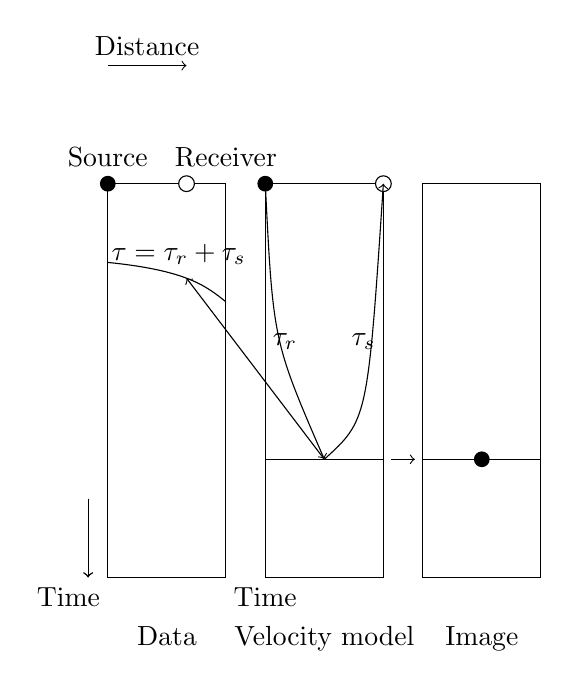
\begin{tikzpicture}[scale=1.0][stealth]
% Time section  
  \draw (0,0) rectangle +(1.5,5);
  \fill (0.0,5.0) circle (0.1) ;
  \draw (0.0,5.1) node[above]{Source};
  \fill[white] (1.0,5.0) circle (0.1) ;
  \draw (1.0,5.0) circle (0.1) ;
  \draw (1.5,5.1) node[above]{Receiver};
  \draw (0,4) .. controls (1.0,3.9) and (1.25,3.7).. (1.5,3.5);
  \draw (0.5,6.5) node[above]{Distance};
  \draw (-0.5,0) node[below]{Time};
  \draw[->] (0,6.5) -- (1,6.5);  
  \draw[->] (-0.25,1) -- (-0.25,0);  
  \draw (0.75,-0.5) node[below]{Data};
% Depth model
  \draw (2,0) rectangle +(1.5,5);
  \fill (2,0) +(0.0,5.0) circle (0.1) ;
  \fill[white] (2,0) +(1.5,5.0) circle (0.1) ;
  \draw (2,0) +(1.5,5.0) circle (0.1) ;
  \draw (2.0,0) node[below]{Time};
  %\draw[->] (0,5.5) -- (1,5.5);  
  \draw[->] (-0.25,1) -- (-0.25,0);  
%
% Rays
% \draw[->] (2.0,5) -- (2.75,1.5);
% \draw[->] (2.75,1.5) -- (3.5,5);

\draw[->] (2.0,5) .. controls (2.1, 3) ..(2.75,1.5);
  \draw[->] (2.75,1.5) .. controls (3.3,2.0) .. (3.5,5);
%
  \draw (2.0,1.5) -- (3.5,1.5);
  \draw (2,0) +(0.75,-0.5) node[below]{Velocity model};
  \draw (2,0) +(1.25,3) node{$\tau_s$};
  \draw (2,0) +(0.25,3) node{$\tau_r$};
  \draw[->] (2.75,1.5) -- (1.0,3.8);
  \draw (0.9,4.1) node{$\tau=\tau_r+\tau_s$};
% Image
  \draw[->] (3.6,1.5) -- (3.9,1.5);
  \draw (4,0) rectangle +(1.5,5);
  \draw (4,0) +(0.75,-0.5) node[below]{Image};
  \draw (4.0,1.5) -- +(1.5,0);
  \fill (4.75,1.5) circle (0.1) ;
\end{tikzpicture}
\caption{Kirchoff time migration}
\label{fig:si-4}
\end{figure}
\end{frame}
%
%------------------------------------------------
\begin{frame}{Common Image Point (CIP) Gathers}
%------------------------------------------------
%
\begin{figure}
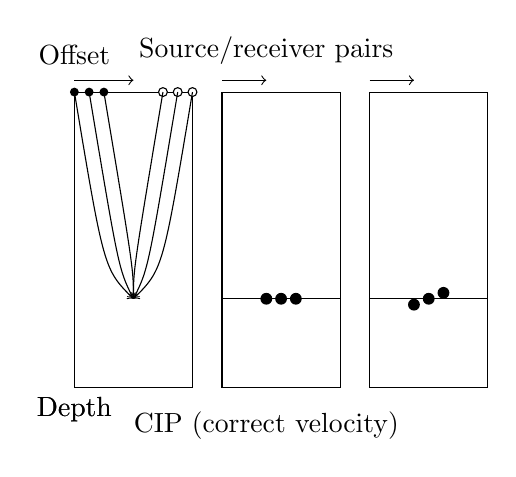
\begin{tikzpicture}[scale=0.75][stealth]
% Depth model outline
  \draw (0,0) rectangle +(2.0,5);
% Annotation on outline
  \draw[->] (0.0,5.2) -- +(1.0,0);
  \draw (0.0,5.3) node[above]{Offset};
  \draw (0.0,0) node[below]{Depth};
% Source point no1
  \fill (0,0) +(0.0,5.0) circle (0.075) ;
% Receiver point no1
  \fill[white] (0,0) +(2.0,5.0) circle (0.075) ;
  \draw (0,0) +(2.0,5.0) circle (0.075) ;
% Source point no2
  \fill (0,0) +(0.25,5.0) circle (0.075) ;
% Receiver point no2
  \fill[white] (0,0) +(1.75,5.0) circle (0.075) ;
  \draw (0,0) +(1.75,5.0) circle (0.075) ;
  \draw (0.0,0) node[below]{Depth};
% Source point no3
  \fill (0,0) +(0.5,5.0) circle (0.075) ;
% Receiver point no3
  \fill[white] (0,0) +(1.5,5.0) circle (0.075) ;
  \draw (0,0) +(1.5,5.0) circle (0.075) ;
% Ray pair no 1
  \draw[->] (0.0,5) .. controls (0.5,2.0) ..(1.0,1.5);
  \draw[->] (2.0,5) .. controls (1.5,2.0) ..(1.0,1.5);
% Ray pair no 2
  \draw[->] (0.25,5) .. controls (0.75,2.0) ..(1.0,1.5);
  \draw[->] (1.75,5) .. controls (1.25,2.0) ..(1.0,1.5);
% Ray pair no 2
  \draw[->] (0.5,5) .. controls (1.0,2.0) ..(1.0,1.5);
  \draw[->] (1.5,5) .. controls (1.0,2.0) ..(1.0,1.5);

% (Correct velocity)
%
% Common image points outline
  \draw (2.5,0) rectangle +(2.0,5);
% Common image points annotation
  \draw (2.5,5.3) +(0.75,0.0) node[above]{Source/receiver pairs};
  \draw[->] (2.5,5.2) -- +(0.75,0.0);
  \draw (2.5,0) +(0.75,-0.25) node[below]{CIP (correct velocity)};
% Horiz line
  \draw (2.5,1.5) -- (4.5,1.5);
% Common image point no 1 (center)
  \fill (3.5,1.5) circle (0.1) ;
% Common image point no 2 (left)
  \fill (3.25,1.5) circle (0.1) ;
% Common image point no 1 (right)
  \fill (3.75,1.5) circle (0.1) ;

%
% (Wrong velocity)
%
% Common image points outline
  \draw (5.0,0) rectangle +(2.0,5);
% Common image points annotation
  %\draw (5.0,5.3) +(0.75,0.0) node[above]{Source/receiver pairs};
  \draw[->] (5.0,5.2) -- +(0.75,0.0);
%  \draw (5.0,0) +(0.75,-0.25) node[below]{CIP (incorrect velocity)};
% Horiz line
  \draw (5.0,1.5) -- +(2.0,0.0);
% Common image point no 1 (center)
  \fill (6.0,1.5) circle (0.1) ;
% Common image point no 2 (left)
  \fill (5.75,1.4) circle (0.1) ;
% Common image point no 1 (right)
  \fill (6.25,1.6) circle (0.1) ;
\end{tikzpicture}
\caption{Common image-point gather}
\label{fig:si-300}
\end{figure}
\end{frame}
%==============================================
\begin{frame}{Kirchhoff time migration}
%==============================================
%
\begin{figure}
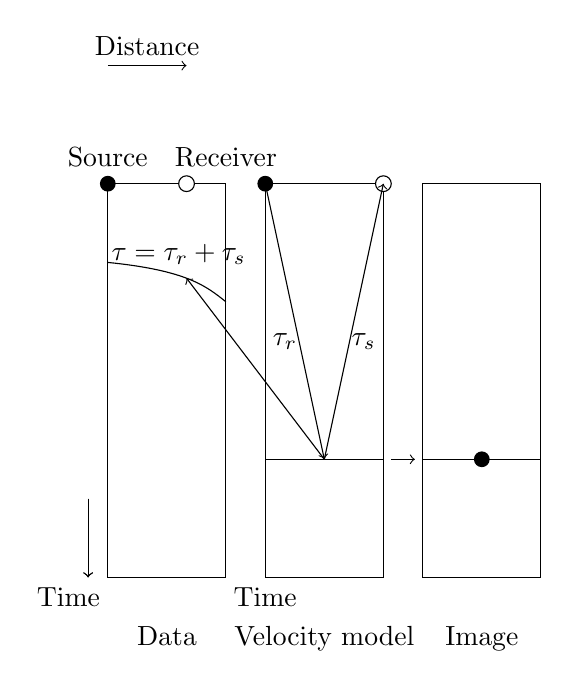
\begin{tikzpicture}[scale=1.0][stealth]
% Time section  
  \draw (0,0) rectangle +(1.5,5);
  \fill (0.0,5.0) circle (0.1) ;
  \draw (0.0,5.1) node[above]{Source};
  \fill[white] (1.0,5.0) circle (0.1) ;
  \draw (1.0,5.0) circle (0.1) ;
  \draw (1.5,5.1) node[above]{Receiver};
  \draw (0,4) .. controls (1.0,3.9) and (1.25,3.7).. (1.5,3.5);
  \draw (0.5,6.5) node[above]{Distance};
  \draw (-0.5,0) node[below]{Time};
  \draw[->] (0,6.5) -- (1,6.5);  
  \draw[->] (-0.25,1) -- (-0.25,0);  
  \draw (0.75,-0.5) node[below]{Data};
% Depth model
  \draw (2,0) rectangle +(1.5,5);
  \fill (2,0) +(0.0,5.0) circle (0.1) ;
  \fill[white] (2,0) +(1.5,5.0) circle (0.1) ;
  \draw (2,0) +(1.5,5.0) circle (0.1) ;
  \draw (2.0,0) node[below]{Time};
  %\draw[->] (0,5.5) -- (1,5.5);  
  \draw[->] (-0.25,1) -- (-0.25,0);  
%
% Rays
 \draw[->] (2.0,5) -- (2.75,1.5);
 \draw[->] (2.75,1.5) -- (3.5,5);

  \draw (2.0,1.5) -- (3.5,1.5);
  \draw (2,0) +(0.75,-0.5) node[below]{Velocity model};
  \draw (2,0) +(1.25,3) node{$\tau_s$};
  \draw (2,0) +(0.25,3) node{$\tau_r$};
  \draw[->] (2.75,1.5) -- (1.0,3.8);
  \draw (0.9,4.1) node{$\tau=\tau_r+\tau_s$};
% Image
  \draw[->] (3.6,1.5) -- (3.9,1.5);
  \draw (4,0) rectangle +(1.5,5);
  \draw (4,0) +(0.75,-0.5) node[below]{Image};
  \draw (4.0,1.5) -- +(1.5,0);
  \fill (4.75,1.5) circle (0.1) ;
\end{tikzpicture}
\caption{Kirchoff time migration}
\label{fig:si-5}
\end{figure}
\end{frame}
%----------------------------------------------------------
\begin{frame}{Velocity estimation for time migration}
%----------------------------------------------------------
Classical velocity analysis is based on the 
traveltime formula 
%
\begin{eqnarray}
\tau(h)=\sqrt{t^2_0+4h^2/c^2},
\label{eq:si-600}
\end{eqnarray}
%
and the nmo-correction defined by
\begin{eqnarray}
\Delta \tau =\tau(h)-t_0.
\label{eq:si-601}
\end{eqnarray}
\end{frame}
%----------------------------------------------------------
\begin{frame}{Velocity estimation for time migration}
%----------------------------------------------------------
\begin{figure}
\includegraphics[width=0.6\textwidth]{Fig/si-fig-nmo-low.pdf}
\caption{Cmp gather (left) and nmo-corrected cmp gather with too low velocity.}
\label{fig:si-fig-nmo-low}
\end{figure}
%
\end{frame}
%----------------------------------------------------------
\begin{frame}{Velocity estimation for time migration}
%----------------------------------------------------------
%
\begin{figure}
\includegraphics[width=0.6\textwidth]{Fig/si-fig-nmo-high.pdf}
\caption{Cmp gather (left) and nmo-corrected cmp gather with too high velocity.}
\label{fig:si-fig-nmo-high}
\end{figure}
%
\end{frame}
%----------------------------------------------------------
\begin{frame}{Velocity estimation for time migration}
%----------------------------------------------------------
Maximizing stack power to find velocity
%
\begin{eqnarray}
   e_s= \sum_{t,h} p^2(h,t),
\label{eq:si-602}
\end{eqnarray}
where the summation is over all times $t$ and offsets $h$.

Minimize differential semblance
%
\begin{eqnarray}
  e_d = \sum_{t,h} [d_h p(h,t)]^2,
\label{eq:si-603}
\end{eqnarray}
where $d_h$ denotes differentiation in the
offset direction.
\begin{itemize}
\item Velocity analysis  always on migrated data
\item Initial crude velocity function must be known
\item New migration performed after velocity analysis
\item Reduced noise level on migrated data
\end{itemize}
\end{frame}
%------------------------------------------------
\begin{frame}{Velocity analysis for depth migration}
%------------------------------------------------
%
\begin{figure}
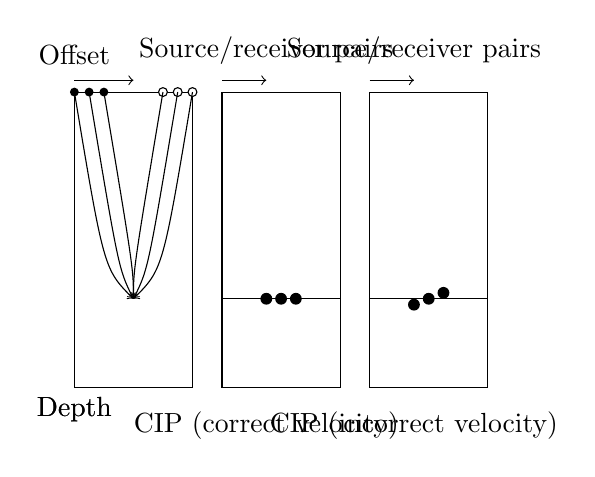
\begin{tikzpicture}[scale=0.75][stealth]
% Depth model outline
  \draw (0,0) rectangle +(2.0,5);
% Annotation on outline
  \draw[->] (0.0,5.2) -- +(1.0,0);
  \draw (0.0,5.3) node[above]{Offset};
  \draw (0.0,0) node[below]{Depth};
% Source point no1
  \fill (0,0) +(0.0,5.0) circle (0.075) ;
% Receiver point no1
  \fill[white] (0,0) +(2.0,5.0) circle (0.075) ;
  \draw (0,0) +(2.0,5.0) circle (0.075) ;
% Source point no2
  \fill (0,0) +(0.25,5.0) circle (0.075) ;
% Receiver point no2
  \fill[white] (0,0) +(1.75,5.0) circle (0.075) ;
  \draw (0,0) +(1.75,5.0) circle (0.075) ;
  \draw (0.0,0) node[below]{Depth};
% Source point no3
  \fill (0,0) +(0.5,5.0) circle (0.075) ;
% Receiver point no3
  \fill[white] (0,0) +(1.5,5.0) circle (0.075) ;
  \draw (0,0) +(1.5,5.0) circle (0.075) ;
% Ray pair no 1
  \draw[->] (0.0,5) .. controls (0.5,2.0) ..(1.0,1.5);
  \draw[->] (2.0,5) .. controls (1.5,2.0) ..(1.0,1.5);
% Ray pair no 2
  \draw[->] (0.25,5) .. controls (0.75,2.0) ..(1.0,1.5);
  \draw[->] (1.75,5) .. controls (1.25,2.0) ..(1.0,1.5);
% Ray pair no 2
  \draw[->] (0.5,5) .. controls (1.0,2.0) ..(1.0,1.5);
  \draw[->] (1.5,5) .. controls (1.0,2.0) ..(1.0,1.5);

% (Correct velocity)
%
% Common image points outline
  \draw (2.5,0) rectangle +(2.0,5);
% Common image points annotation
  \draw (2.5,5.3) +(0.75,0.0) node[above]{Source/receiver pairs};
  \draw[->] (2.5,5.2) -- +(0.75,0.0);
  \draw (2.5,0) +(0.75,-0.25) node[below]{CIP (correct velocity)};
% Horiz line
  \draw (2.5,1.5) -- (4.5,1.5);
% Common image point no 1 (center)
  \fill (3.5,1.5) circle (0.1) ;
% Common image point no 2 (left)
  \fill (3.25,1.5) circle (0.1) ;
% Common image point no 1 (right)
  \fill (3.75,1.5) circle (0.1) ;

%
% (Wrong velocity)
%
% Common image points outline
  \draw (5.0,0) rectangle +(2.0,5);
% Common image points annotation
  \draw (5.0,5.3) +(0.75,0.0) node[above]{Source/receiver pairs};
  \draw[->] (5.0,5.2) -- +(0.75,0.0);
  \draw (5.0,0) +(0.75,-0.25) node[below]{CIP (incorrect velocity)};
% Horiz line
  \draw (5.0,1.5) -- +(2.0,0.0);
% Common image point no 1 (center)
  \fill (6.0,1.5) circle (0.1) ;
% Common image point no 2 (left)
  \fill (5.75,1.4) circle (0.1) ;
% Common image point no 1 (right)
  \fill (6.25,1.6) circle (0.1) ;
\end{tikzpicture}
\caption{Common image-point gather}
\label{fig:si-300}
\end{figure}
\end{frame}
%------------------------------------------------
\begin{frame}{Velocity analysis for depth migration}
%------------------------------------------------
\begin{itemize}
  \item Minimize differential semblance on common-image-point gathers
  \item Kirchhoff migration: MVA
  \item Reverse-time or Wave-equation migration: WEMVA
\end{itemize}
\end{frame}
%
%------------------------------------------------
\begin{frame}{Velocity analysis for depth migration}
%------------------------------------------------
\begin{figure}
\includegraphics[width=0.75\textwidth]{Fig/si-fig-500.pdf}
\includegraphics[width=0.75\textwidth]{Fig/si-fig-501.pdf}
\includegraphics[width=0.75\textwidth]{Fig/si-fig-502.pdf}
\caption{Initial velocity model (top), Model estimated using wave-equation migration 
         velocity analysis (bottom) and velocity estimated using ray based migration
         velocity analysis (MVA)(bottom).}
\label{fig:si-fig-301}
\end{figure}
\end{frame}
%
%
%------------------------------------------------
\begin{frame}{Velocity analysis for depth migration}
%------------------------------------------------
\begin{figure}
\includegraphics[width=0.75\textwidth]{Fig/si-fig-503.pdf}
\caption{Image point gather for the initial velocity model (left), 
         the velocity model estimated using WEMVA (middle) and the MVA velocity model (right).}
\label{fig:si-fig-302}
\end{figure}
\end{frame}
%
%------------------------------------------------
\begin{frame}{Velocity analysis for depth migration}
%------------------------------------------------
%
\begin{figure}
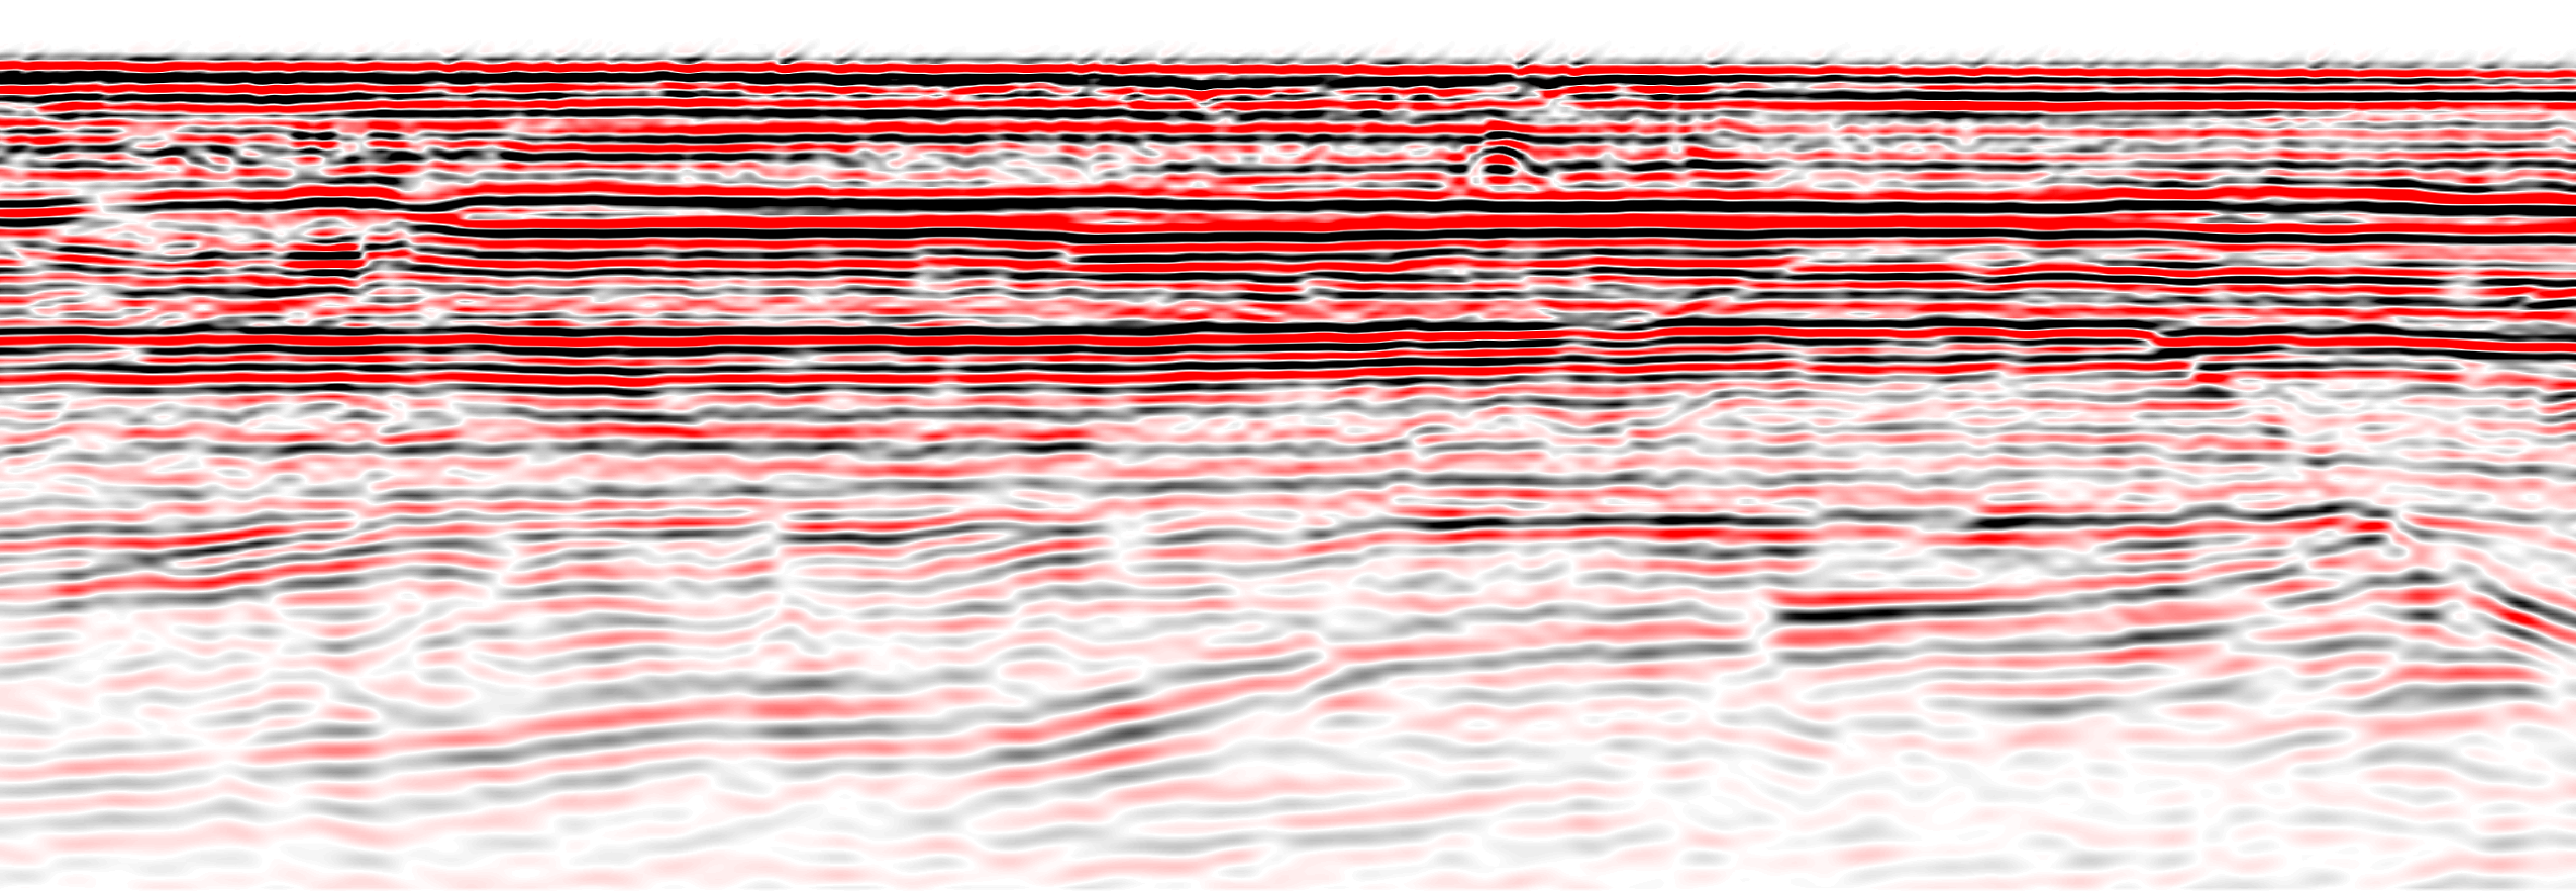
\includegraphics[width=0.6\textwidth]{Fig/si-fig-504.pdf}
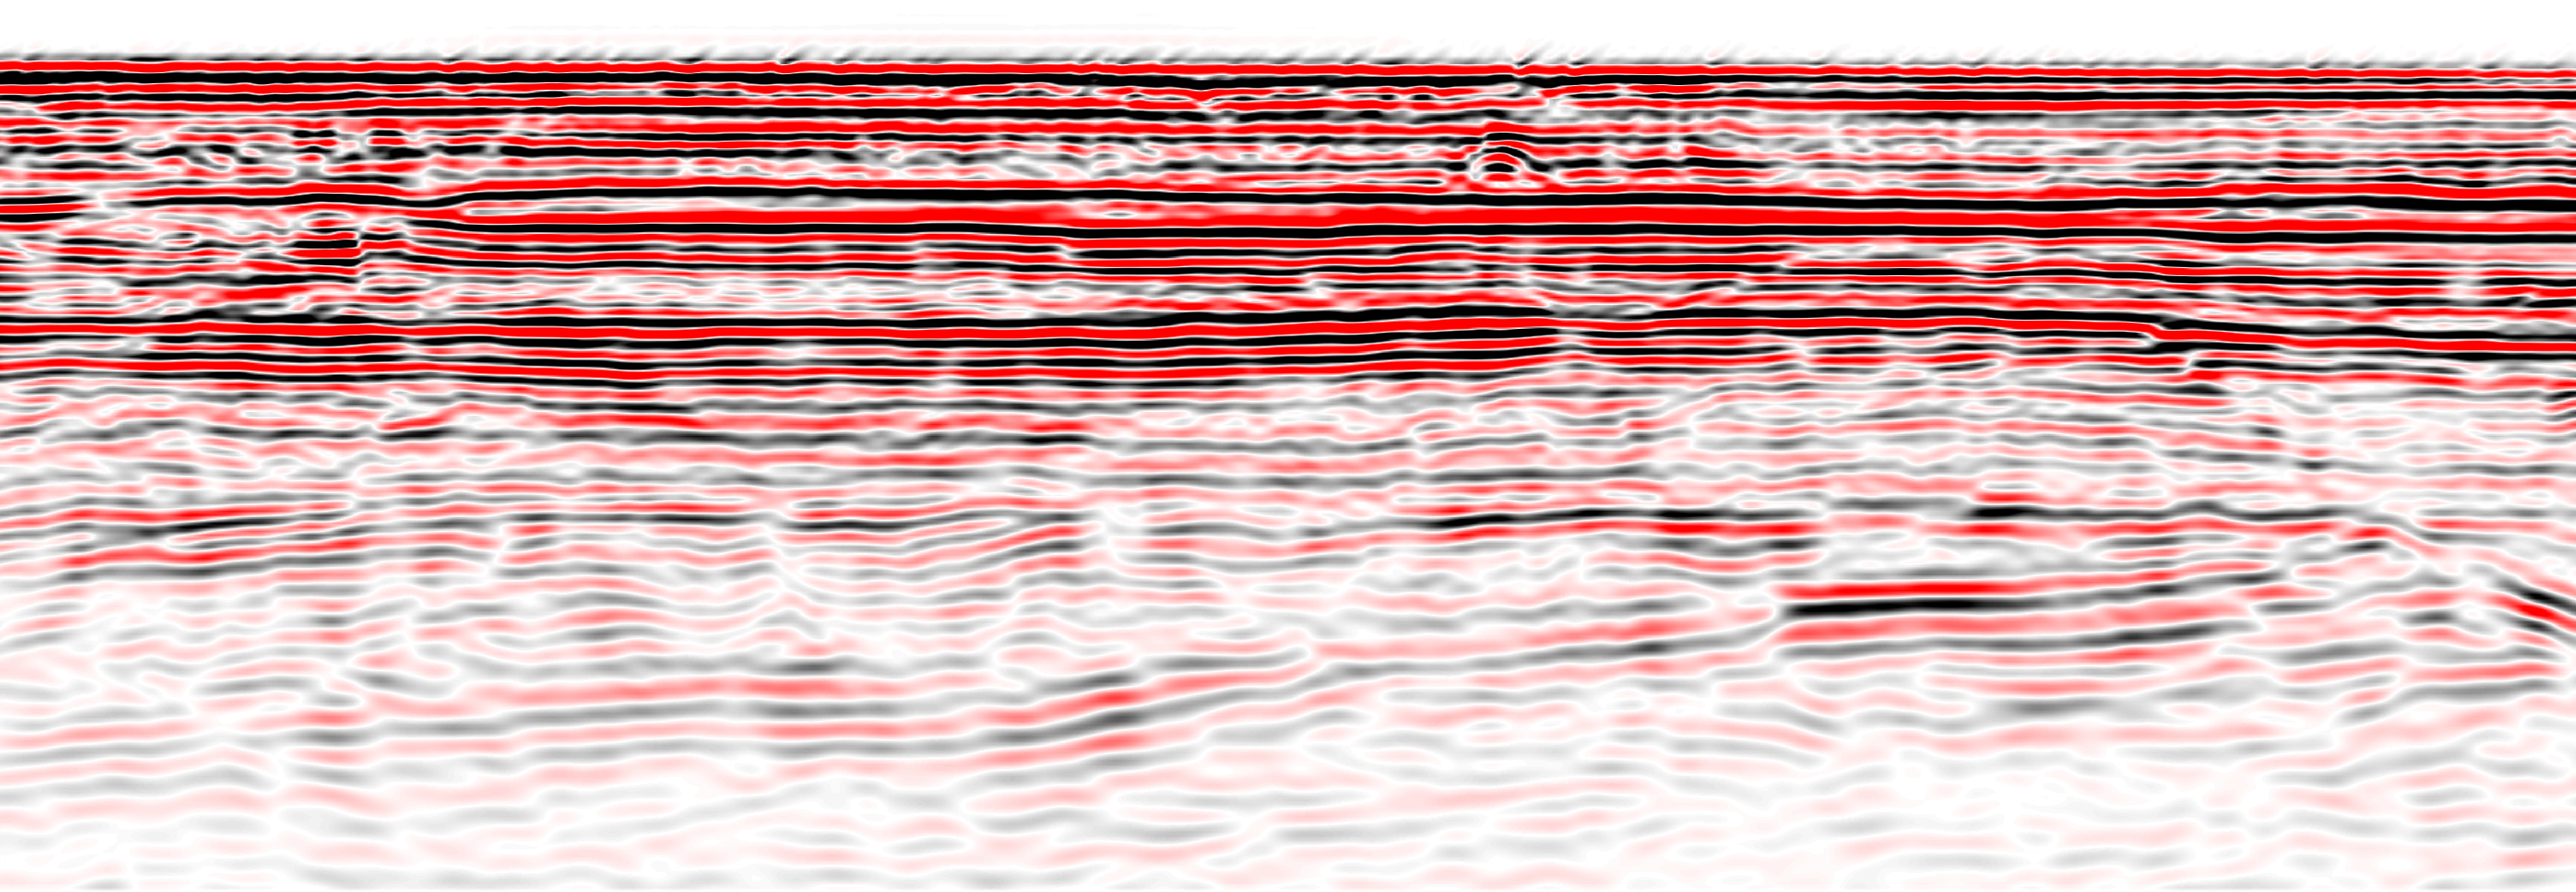
\includegraphics[width=0.6\textwidth]{Fig/si-fig-505.pdf}
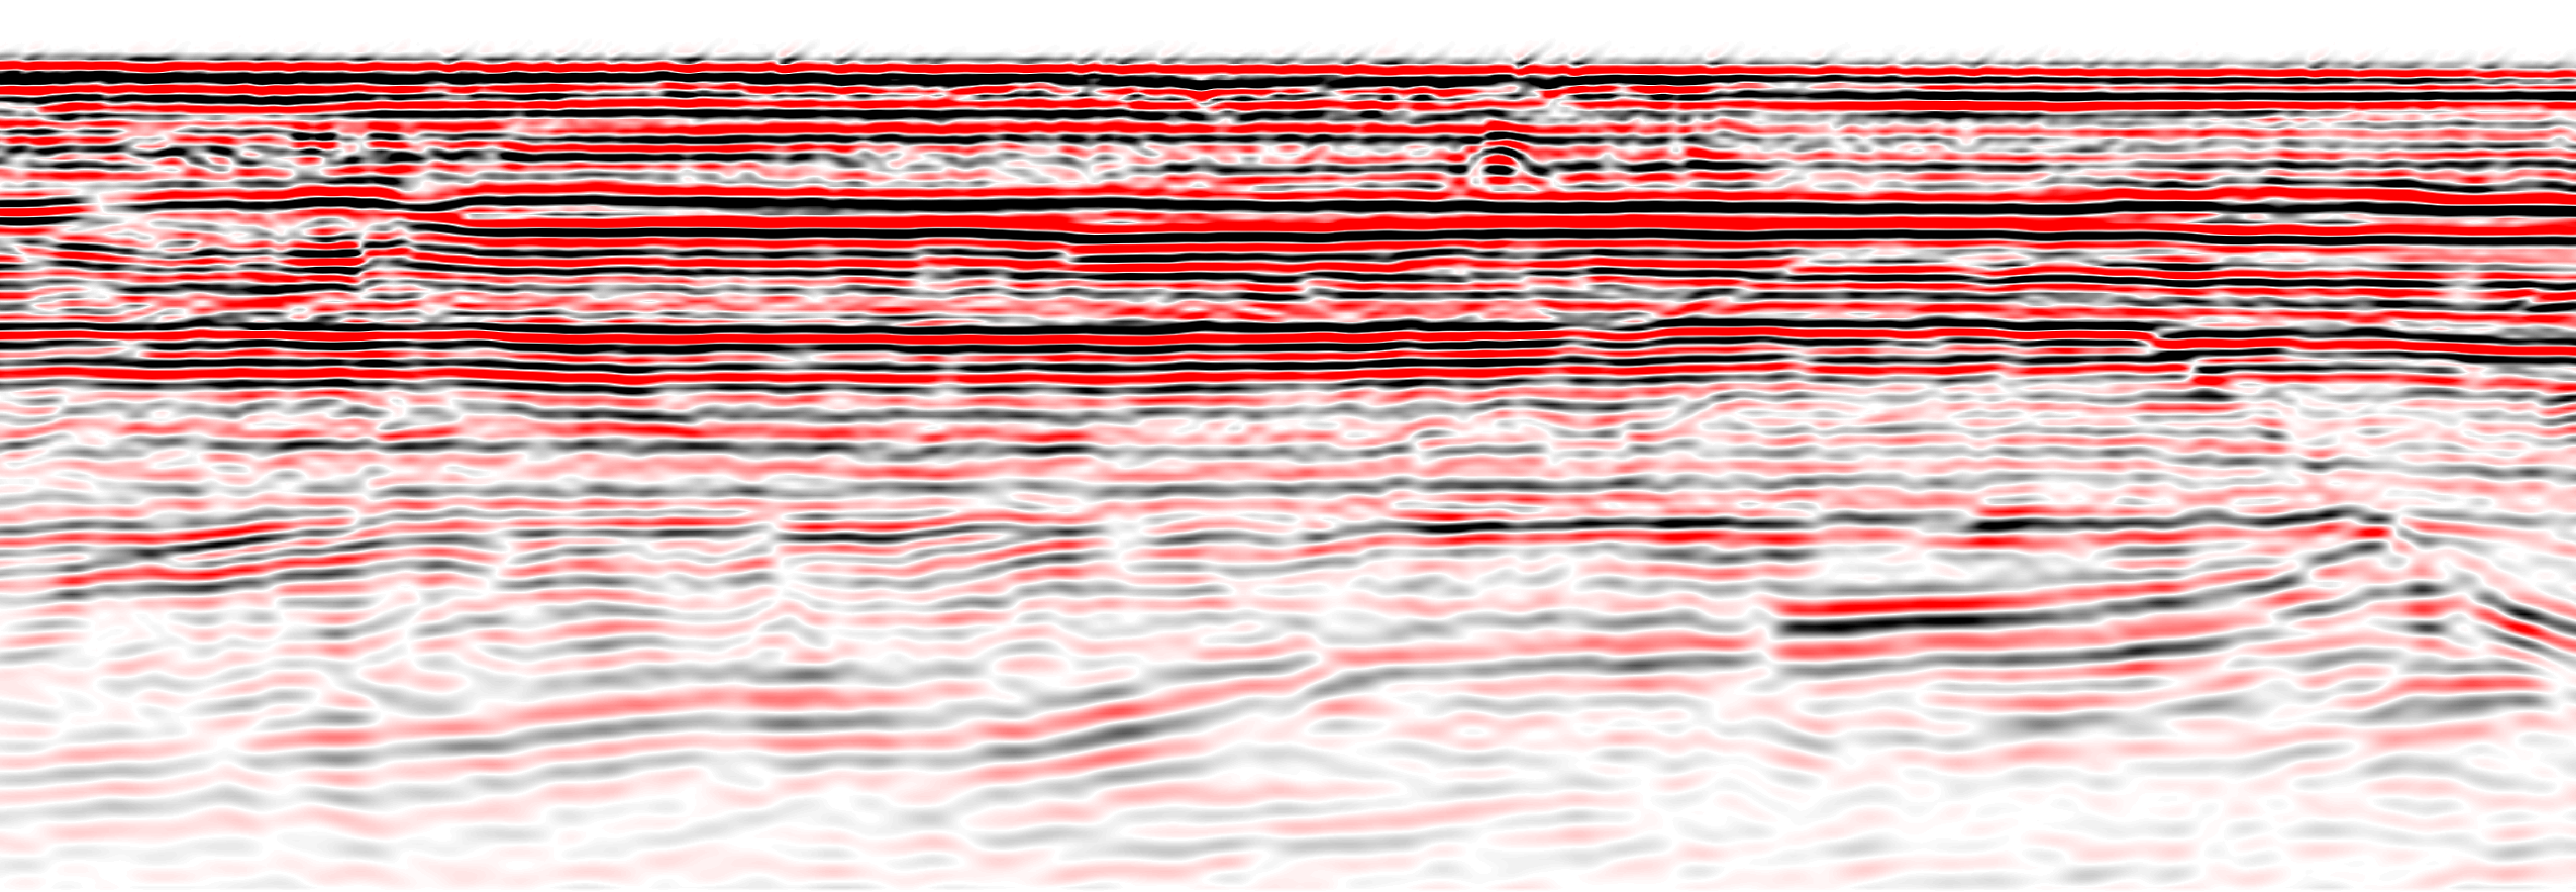
\includegraphics[width=0.6\textwidth]{Fig/si-fig-506.pdf}
\caption{Seismic sections corresponding to the inital velocity model (top)
         the velocity model using WEMVA (middle) and the velocity model using MVA (bottom).}
\label{fig:si-fig-303}
\end{figure}
\end{frame}
%------------------------------------------------------
\begin{frame}{Full-waveform Inversion}
%---------------------------------------------------------
Minimize difference between simulation and observed data
%
\begin{eqnarray}
  e_l = \sum_{r,t}[p(\xx_r,t)-p^{obs}(\xx_r,t)]^2,
\end{eqnarray}
where the summation is over receivers and time.
\end{frame}
%------------------------------------------------------
\begin{frame}{Full-waveform Inversion}
%---------------------------------------------------------
%
\begin{figure}
\includegraphics[width=0.75\textwidth]{Fig/si-fig-511.pdf}
\caption{Velocity model for the Gullfaks synthetic dataset estimated using full waveform inversion}.
\label{fig:si-fig-304}
\end{figure}
\end{frame}
%
%------------------------------------------------------
\begin{frame}{Full-waveform Inversion}
%---------------------------------------------------------
\begin{figure}
\includegraphics[width=0.75\textwidth]{Fig/si-fig-510.pdf}
\caption{Velocity model for the Gullfaks synthetic dataset estimated using WEMVA}.
\label{fig:si-fig-305}
\end{figure}
%
\end{frame}
%
%------------------------------------------------------
\begin{frame}{Full-waveform Inversion}
%---------------------------------------------------------
\begin{figure}
\includegraphics[width=0.75\textwidth]{Fig/si-fig-400.pdf}
\caption{True velocity model for the Gullfaks synthetic dataset.}.
\label{fig:si-fig-400}
\end{figure}
%
\end{frame}
%
\end{document}
\end{document}
